%   ------------------------------------------------------------------------
\FloatBarrier
\section{OpenArt.AI}
\label{s.OpenArtApendice}

\begin{figure}[htbp]
    \centering
    \begin{minipage}{0.45\textwidth}
    \centering
    \caption{\small Tela módulos do OpenArt.AI}
    \label{fig:openArtModulos}
    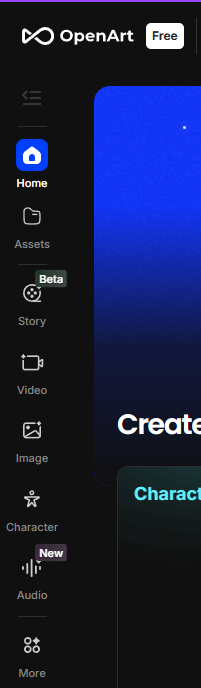
\includegraphics[width=0.7\linewidth]{figs/OpenArtAI/telaOpenArt.PNG}
    \legend{\small Fonte: Elaborada pela autora.}
    \end{minipage}
    \hfill
    \begin{minipage}{0.45\textwidth}
    \centering
    \caption{\small Funcionalidades do módulo de vídeo do OpenArt.AI}
    \label{fig:openArtModuloVideo}
    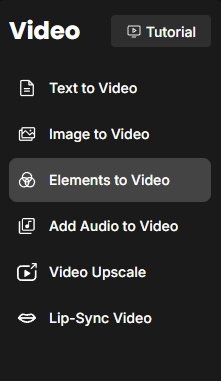
\includegraphics[width=0.7\linewidth]{figs/OpenArtAI/telaVideoModulos.PNG}
    \legend{\small Fonte: Elaborada pela autora.}
    \end{minipage}
\end{figure}

\begin{figure}[htbp]
    \centering
    \caption{\small Modelos de IA para geração de vídeo no OpenArt.AI}
    \label{fig:openArtModelosVideo}
    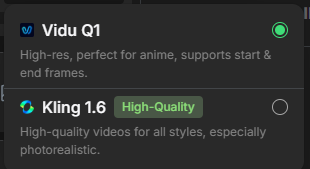
\includegraphics[width=0.5\linewidth]{figs/OpenArtAI/opcoesModeloVideo.PNG}
    \legend{\small Fonte: Elaborada pela autora.}
\end{figure}


\begin{figure}[htbp]
    \centering
    \caption{\small Geração de vídeo no OpenArt.AI}
    \label{fig:openArtVideo}
    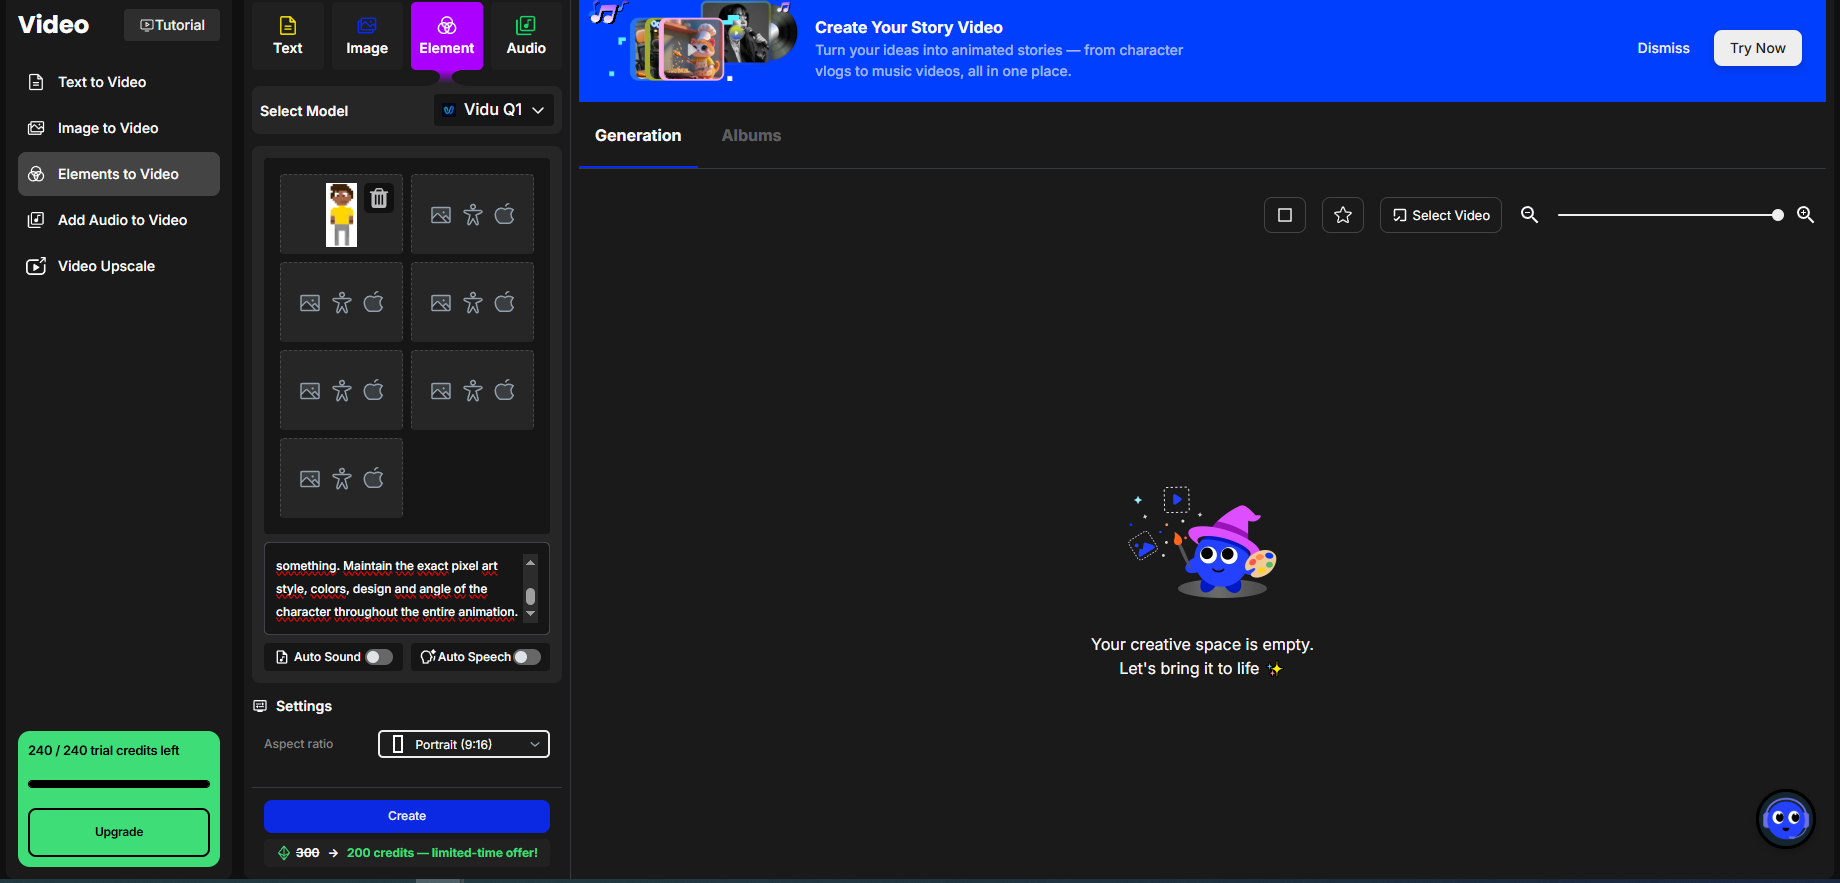
\includegraphics[width=1\linewidth]{figs/OpenArtAI/telaVideo.PNG}
    \legend{\small Fonte: Elaborada pela autora.}
\end{figure}

\begin{figure}[htbp]
    \centering
    \caption{\small Funcionalidades do módulo de imagem do OpenArt.AI}
    \label{fig:openArtModuloImagem}
    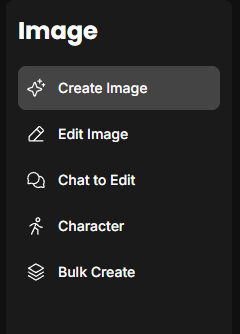
\includegraphics[width=0.3\linewidth]{figs/OpenArtAI/telaImagemModulos.PNG}
    \legend{\small Fonte: Elaborada pela autora.}
\end{figure}

\begin{figure}[htbp]
    \centering
    \caption{\small Modelos para editar imagem do OpenArt.AI}
    \label{fig:openArtModelosImagem}
    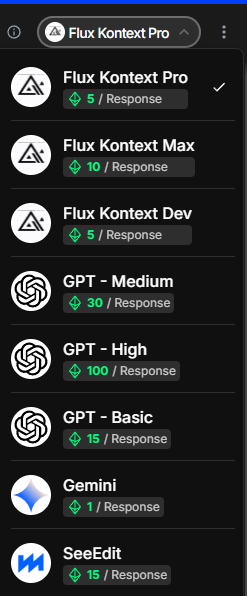
\includegraphics[width=0.3\linewidth]{figs/OpenArtAI/opcoesModeloEdit.PNG}
    \legend{\small Fonte: Elaborada pela autora.}
\end{figure}

\begin{figure}[htbp]
    \centering
    \caption{\small Tela geração de imagem com o modelo SeedEdit no OpenArt.AI}
    \label{fig:openArtModeloSeedEdit}
    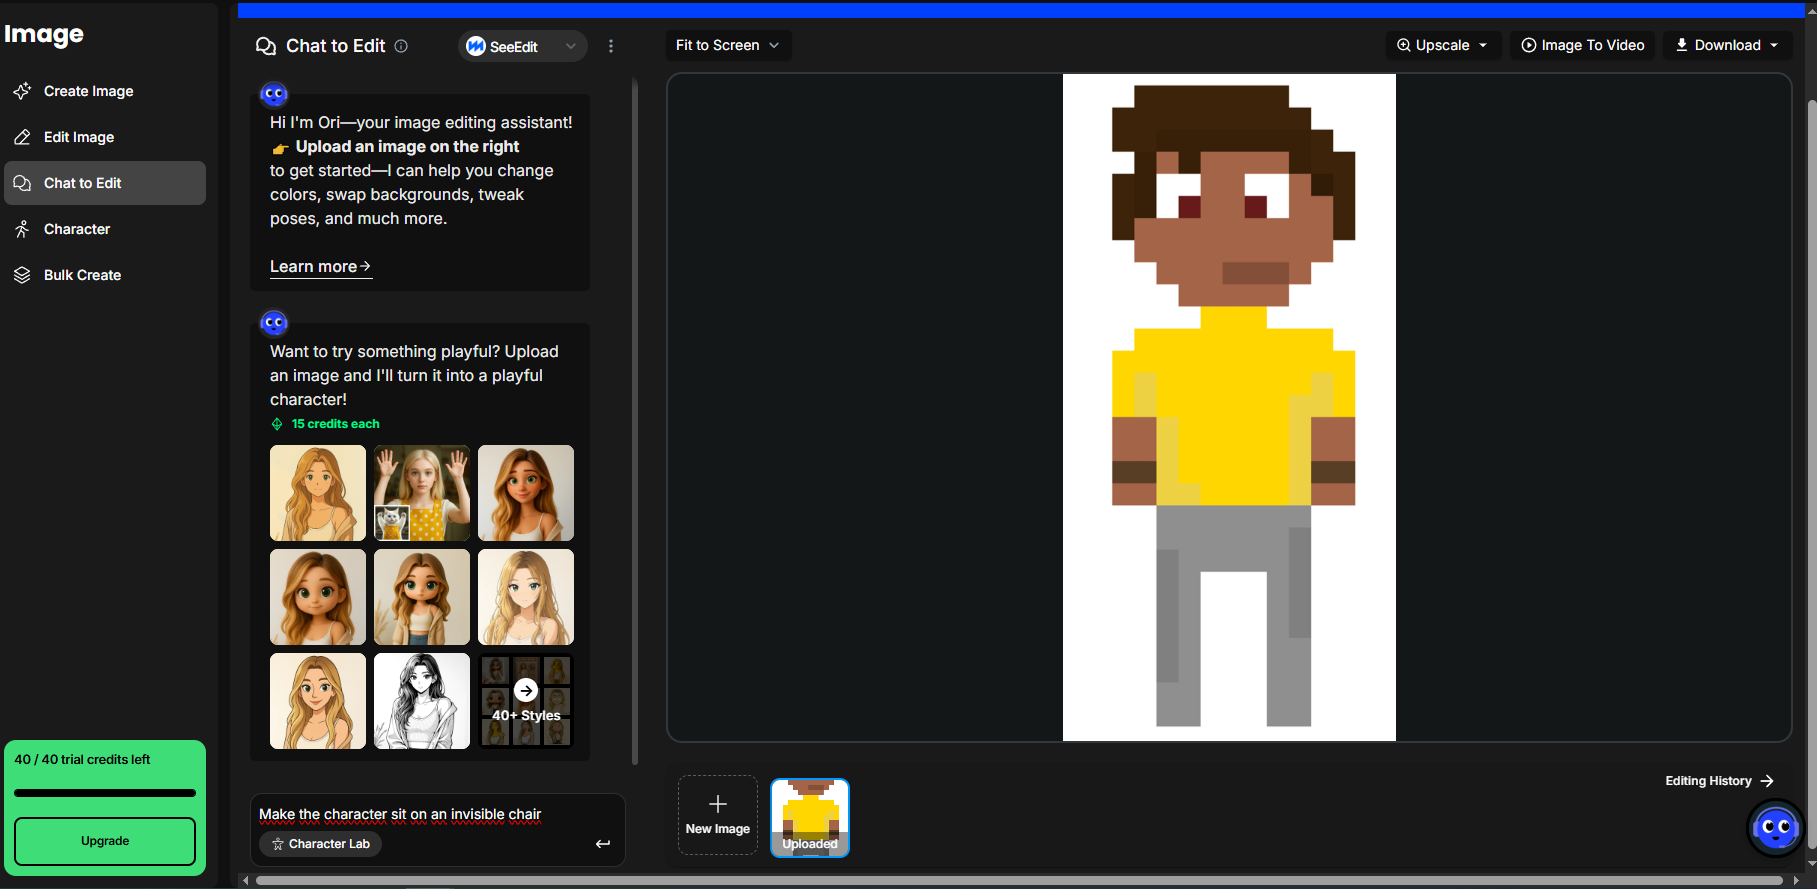
\includegraphics[width=1\linewidth]{figs/OpenArtAI/telaSeeEdit.PNG}
    \legend{\small Fonte: Elaborada pela autora.}
\end{figure}


\begin{figure}[htbp]
    \centering
    \caption{\small Tela geração de imagem com o modelo Flux Kontext no OpenArt.AI}
    \label{fig:openArtModeloFluxContext}
    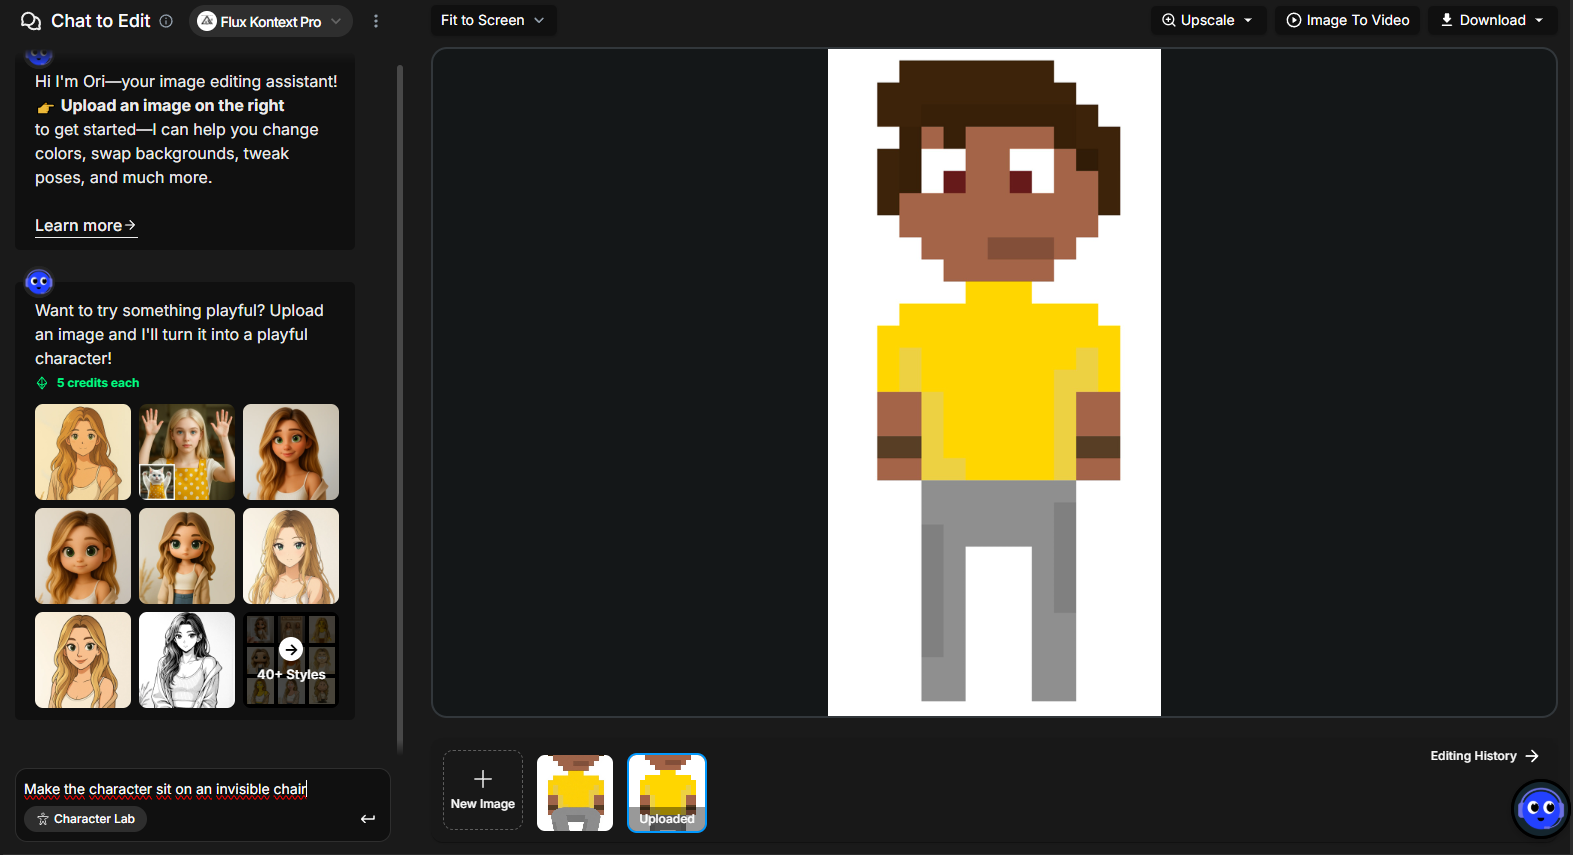
\includegraphics[width=1\linewidth]{figs/OpenArtAI/telafluxKontextPro.PNG}
    \legend{\small Fonte: Elaborada pela autora.}
\end{figure}

\begin{figure}[htbp]
    \centering
    \caption{\small Tela geração de imagem com o modelo Gemini no OpenArt.AI}
    \label{fig:openArtModeloGemini}
    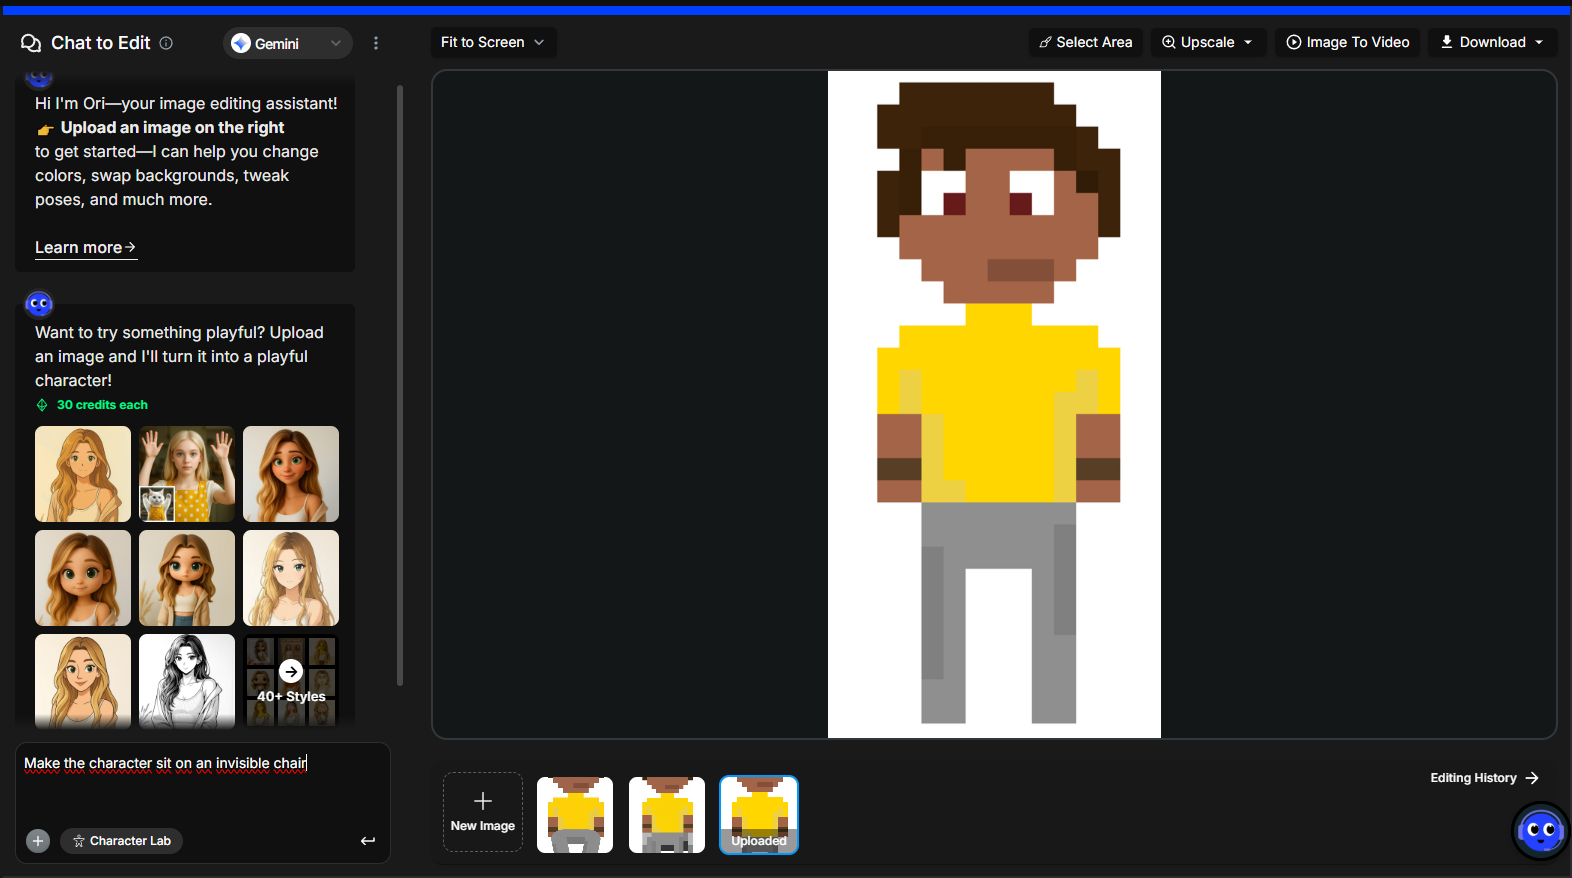
\includegraphics[width=1\linewidth]{figs/OpenArtAI/telaGemini.PNG}
    \legend{\small Fonte: Elaborada pela autora.}
\end{figure}

\begin{figure}[htbp]
    \centering
    \caption{\small Tela geração de imagem com o modelo GPT no OpenArt.AI}
    \label{fig:openArtModeloGPT}
    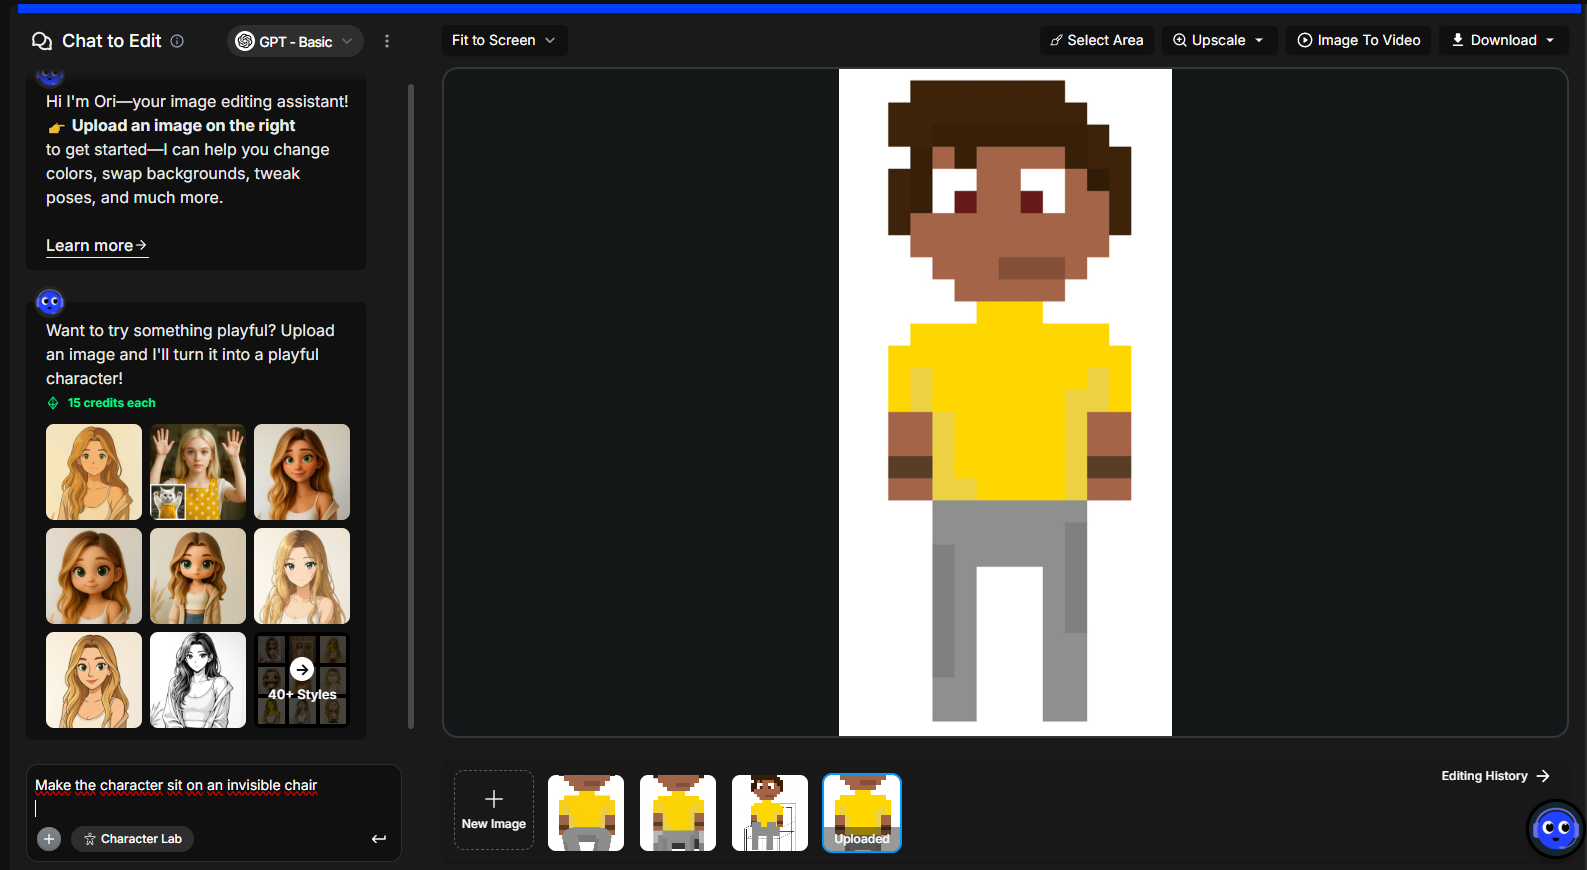
\includegraphics[width=1\linewidth]{figs/OpenArtAI/telaGPT.PNG}
    \legend{\small Fonte: Elaborada pela autora.}
\end{figure}